\section[Wykład 6: 30-III-2017 - Temat: Przepływy w sieciach]{Temat: Przepływy w sieciach}
\subsection{Sieć}
\begin{definition}[Sieć]
Siecią nazywamy piątkę: $$S=(V,A,s,t,c)$$ gdzie
\begin{itemize}
\item[$V,A$] $\rightarrow $ graf skierowany o zbiorze wierzchołków $V$ i zbiorze strzałek $A$,
\item[$s$] $\rightarrow $ $s\in V$ wyróżniony wierzchołek nazywany \textbf{Źródłem},
\item[$t$] $\rightarrow $ $t\in V$ wyróżniony wierzchołek nazywany \textbf{Ujściem},
\item[$c$] $\rightarrow $ $c:A\rightarrow \mathbb{R} _+\cup \{0\}$ funkcja przyporządkowująca strzałkom wartość $\mathbb{R} _+\cup \{0\}$ nazywamy \textbf{funkcją pojemności}
\end{itemize}
\end{definition}
\begin{definition}[Graf skierowany]
Graf $D=(V,A)$ gdzie 
\begin{itemize}
\item[$V$] $\rightarrow $ zbiór wierzchołków,
\item[$A$] $\rightarrow $ $A\subseteq \{(v,w):v,w\in V\}$
\end{itemize}
\end{definition}
\begin{definition}[Przepływ sieci]
Przepływem sieci $S=(V,A,s,t,c)$ nazywamy funkcję $$f:A\rightarrow \mathbb{R}_+\cup \{0\}$$ spełniająca następujące warunki:
\begin{enumerate}[label=\alph*)]
\item $\forall _{a\in A}: 0\leq f(a)\leq c(a)$
\item $\forall _{v\in V,\, v\neq s,\, t}$
$$\sum _{\vec{wv}\in A}f(\vec{wv})=\sum _{\vec{vu}}f(\vec{vu})$$
\end{enumerate}
\end{definition}
\begin{definition}[Wartość przepływu]
Wartość przepływu $f$ jest zdefiniowana jako:
$$\mathsf{val}(f)=\sum _{\vec{sv}\in A}f(\vec{sv})=\sum _{\vec{ut}\in A} f(\vec{ut})$$
\end{definition}

\begin{algorithm*}
\caption{alg:Ford-Fulkerson}\label{alg:Ford-Fulkerson}
\begin{algorithmic}[1]
\Procedure{Ford-Fulkerson}{}
\State Zaczynamy od dowolnego przepływu $f$
\While{Jeśli jeszcze można}
	\State Modyfikujemy przepływ zamieniając go na $f'$ żeby $$\mathsf{val}(f')>\mathsf{val}(f)$$
    \State $f=f'$
\EndWhile
\EndProcedure
\end{algorithmic}
\end{algorithm*}

\begin{example*}[Znajdź przepływ n największej wartości $\mathsf{val}(f)$] Przykład zaprezentowany jako rysunki:\newline
\begin{minipage}{0.45\textwidth}
\begin{figure}[H]
\centering
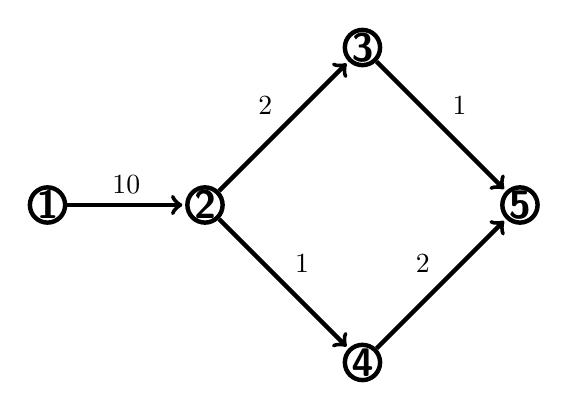
\begin{tikzpicture}[shorten >=1pt, auto, node distance=3cm, ultra thick,main node/.style={circle,draw,minimum size=.4cm,inner sep=0pt]}]%fill=black,
\begin{scope}[every node/.style={font=\sffamily\Large\bfseries}]
\node[main node] (v1) at (0,0) {1};
\node[main node] (v2) at (2,0) {2};
\node[main node] (v3) at (4,2) {3};
\node[main node] (v4) at (4,-2) {4};
\node[main node] (v5) at (6,0) {5};
%\node[main node] (v) at (,) {};
\end{scope}
\begin{scope}[every edge/.style={draw=black,ultra thick}]
\draw[->]  (v1) edge node{$10$} (v2);
\draw[->]  (v2) edge node{$2$} (v3);
\draw[->]  (v2) edge node{$1$} (v4);
\draw[->]  (v3) edge node{$1$} (v5);
\draw[->]  (v4) edge node{$2$} (v5);
%\draw[->]  (v) edge node{} (v);
\end{scope}
\end{tikzpicture}
\caption*{Przykład: $s=1,\ t=3$}
\end{figure}
\end{minipage}

\begin{minipage}{0.95\textwidth}
\begin{figure}[H]
\centering
\begin{tikzpicture}[shorten >=1pt, auto, node distance=3cm, ultra thick,main node/.style={circle,draw,minimum size=.4cm,inner sep=0pt]}]%fill=black,
\begin{scope}[every node/.style={font=\sffamily\Large\bfseries}]
\node[main node] (v1) at (0,0) {1};
\node[main node] (v2) at (2,0) {2};
\node[main node] (v3) at (4,2) {3};
\node[main node] (v4) at (4,-2) {4};
\node[main node] (v5) at (6,0) {5};

%\node[main node] (v) at (,) {};
\end{scope}
\begin{scope}[every edge/.style={draw=black,ultra thick}]
\draw[->]  (v1) edge node{$\overset{2}{10}$} (v2);
\draw[->]  (v2) edge node{$\overset{1}{2}$} (v3);
\draw[->]  (v2) edge node{$\overset{1}{1}$} (v4);
\draw[->]  (v3) edge node{$\overset{1}{1}$} (v5);
\draw[->]  (v4) edge node{$\overset{3}{2}$} (v5);
%\draw[->]  (v) edge node{} (v);
\end{scope}
\end{tikzpicture}
\caption*{Przykład: $s=1,\ t=3$ z zaznaczonym przepływem, powyżej wartości wag}
\end{figure}
\end{minipage}

\begin{minipage}{0.95\textwidth}
\begin{figure}[H]
\centering
\begin{tikzpicture}[shorten >=1pt, auto, node distance=3cm, ultra thick,main node/.style={circle,draw,minimum size=.4cm,inner sep=0pt]}]%fill=black,
\begin{scope}[every node/.style={font=\sffamily\Large\bfseries}]
\node[main node] (v1) at (0,0) {1};
\node[main node] (v2) at (2,0) {2};
\node[main node] (v3) at (4,2) {3};
\node[main node] (v4) at (4,-2) {4};
\node[main node] (v5) at (6,0) {5};

%\node[main node] (v) at (,) {};
\end{scope}
\begin{scope}[every edge/.style={draw=black,ultra thick}]
\draw[->]  (v1) edge node{$\overset{2}{10}$} (v2);
\draw[->]  (v2) edge node{$\overset{0.5}{2}$} (v3);
\draw[->]  (v2) edge node{$\overset{1.5}{1}$} (v4);
\draw[->]  (v3) edge node{$\overset{0.5}{1}$} (v5);
\draw[->]  (v4) edge node{$\overset{1.5}{2}$} (v5);
%\draw[->]  (v) edge node{} (v);
\end{scope}
\end{tikzpicture}
\caption*{Przykład: $s=1,\ t=3$ z zaznaczonym przepływem, powyżej wartości wag}
\end{figure}
\end{minipage}


\begin{figure}[H]
\centering
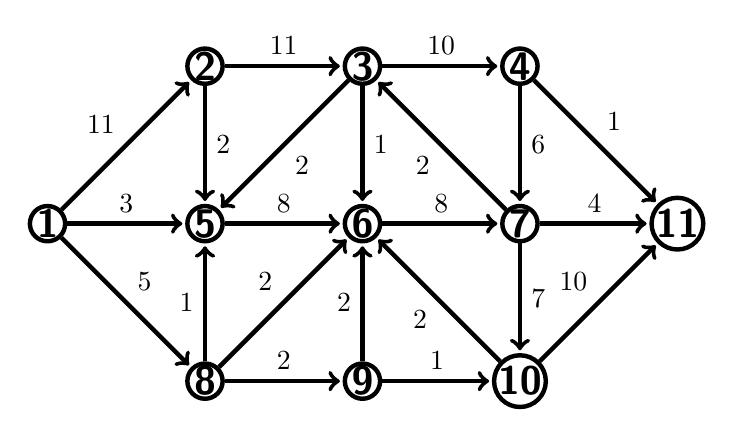
\begin{tikzpicture}[shorten >=1pt, auto, node distance=3cm, ultra thick,main node/.style={circle,draw,minimum size=.4cm,inner sep=0pt]}]%fill=black,
\begin{scope}[every node/.style={font=\sffamily\Large\bfseries}]
\node[main node] (v1) at (0,0) {1};
\node[main node] (v2) at (2,2) {2};
\node[main node] (v3) at (4,2) {3};
\node[main node] (v4) at (6,2) {4};
\node[main node] (v5) at (2,0) {5};
\node[main node] (v6) at (4,0) {6};
\node[main node] (v7) at (6,0) {7};
\node[main node] (v8) at (2,-2) {8};
\node[main node] (v9) at (4,-2) {9};
\node[main node] (v10) at (6,-2) {10};
\node[main node] (v11) at (8,0) {11};
%\node[main node] (v) at (,) {};
\end{scope}
\begin{scope}[every edge/.style={draw=black,ultra thick}]
\draw[->]  (v1) edge node{11} (v2);
\draw[->]  (v1) edge node{3} (v5);
\draw[->]  (v1) edge node{5} (v8);
\draw[->]  (v2) edge node{11} (v3);
\draw[->]  (v2) edge node{2} (v5);
\draw[->]  (v3) edge node{10} (v4);
\draw[->]  (v3) edge node{1} (v6);
\draw[->]  (v3) edge node{2} (v5);
\draw[->]  (v4) edge node{6} (v7);
\draw[->]  (v4) edge node{1} (v11);
\draw[->]  (v5) edge node{8} (v6);
\draw[->]  (v6) edge node{8} (v7);
\draw[->]  (v7) edge node{2} (v3);
\draw[->]  (v7) edge node{4} (v11);
\draw[->]  (v7) edge node{7} (v10);
\draw[->]  (v8) edge node{1} (v5);
\draw[->]  (v8) edge node{2} (v6);
\draw[->]  (v8) edge node{2} (v9);
\draw[->]  (v9) edge node{2} (v6);
\draw[->]  (v9) edge node{1} (v10);
\draw[->]  (v10) edge node{2} (v6);
\draw[->]  (v10) edge node{10} (v11);
%\draw[->]  (v) edge node{} (v);
\end{scope}
\end{tikzpicture}
\caption*{$s=1,\ t=11$}
\end{figure}
\end{example*}

\begin{definition}[Ścieżka nienasycona] ciąg strzałek zaczynających się w $s$ a kończących się w $t$
\begin{figure}[H]
\centering
\begin{tikzpicture}[shorten >=1pt, auto, node distance=3cm, ultra thick,main node/.style={circle,draw,minimum size=.4cm,inner sep=0pt]}]%fill=black,
\begin{scope}[every node/.style={font=\sffamily\Large\bfseries}]
\node[main node] (v1) at (0,0) {$s$};
\node[main node] (v2) at (2,0) {};
\node[main node] (v3) at (4,0) {};
\node[main node] (v4) at (6,0) {};
\node[main node] (v5) at (8,0) {};
\node[main node] (v6) at (10,0) {};
\node[main node] (v7) at (12,0) {$t$};
%\node[main node] (v) at (,) {};
\end{scope}
\begin{scope}[every edge/.style={draw=black,ultra thick}]
\draw[->]  (v1) edge node{$\underset{2=2-0}{2}$} (v2);
\draw[->]  (v2) edge node{$\underset{3=5-2}{5}$} (v3);
\draw[->]  (v4) edge node{1} (v3);
\draw[->]  (v4) edge node{$\underset{2=7-5}{7}$} (v5);
\draw[->]  (v6) edge node{3} (v5);
\draw[->]  (v6) edge node{$\underset{1=2-1}{2}$} (v7);
%\draw[->]  (v) edge node{} (v);
\end{scope}
\end{tikzpicture}
\end{figure}
$$\min \{2,3,1,2,1,1\}=0$$
\end{definition}

\begin{definition}[Cięcie]
Cięciem w sieci $S=(V,A,s,t,c)$ nazywamy podział $V=S\cup \bar{S}$, takie że  $s\in S$, $t\not\in S$, $s\in \bar{S}$.

Pojemnością cięcia $(S,\bar{S})$ nazywamy sumą pojemności wszystkich strzałek z $S$ do $\bar{S}$ to: 
$$\mathsf{cap}(S,\bar{S})=\sum _{v\in S, w\in S}c(\vec{v,w})$$
\end{definition}


\begin{figure}[H]
\centering
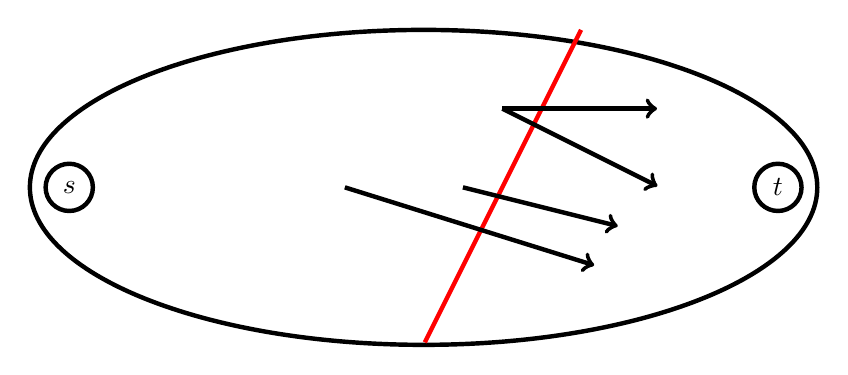
\begin{tikzpicture}[shorten >=1pt, auto, node distance=3cm, ultra thick,main node/.style={circle,draw,minimum size=.4cm,inner sep=0pt]}]%fill=black,
\draw (2,2) ellipse (5cm and 2cm);
\draw[color=red] (4,4) -- (2,0);
\draw[->] (3,3) -> (5,3);
\draw[->] (3,3) -> (5,2); 
\draw[->] (2.5,2) -> (4.5,1.5); 
\draw[->] (1,2) -> (4.2,1); 
\draw (-2.5,2) circle (0.3) node {$s$};
\draw (6.5,2) circle (0.3) node {$t$};
\end{tikzpicture}
\end{figure}

\begin{fact*}
Dla dowolnego przepływu $f$ i dowolnego przecięcia $(S, \bar{S})$
$$\mathsf{val}(f)\leq \mathsf{cap}(S, \bar{S})$$
\end{fact*}

\begin{theorem}[MAX-FLOW-MIN-CUT] Dla każdej serii
$$\max _f \mathsf{val}(f)=\min _{(S, \bar{S})}\mathsf{cap}(S, \bar{S})$$
$$\mathsf{cap}(X,Y)\geq \mathsf{MINCUT}=\mathsf{MAXFLOW}\geq \mathsf{val}(f)$$
\end{theorem}

%--------------------------------------------------